\section{Tracking the Probe on a Deformable Surface}

\subsection{Mesh Following Algorithm}

After calibration, due to deformability and possible measurement errors, our rendered path in the virtual world will have segments that are above or below the virtual surface as shown in Figure \ref{pathsAboveAndBelow}. Because the path was recorded on the real surface, we want a visualization on the virtual surface of the probe's location on the real surface. We will thus do a transformation of the virtual path to better match where the real path traversed. Because we already calibrated the scale of the movements, the transformation will preserve arc length. Because the rotation was already calibrated, the orientation along the surface will be preserved.

\begin{figure}[ht]
\centering
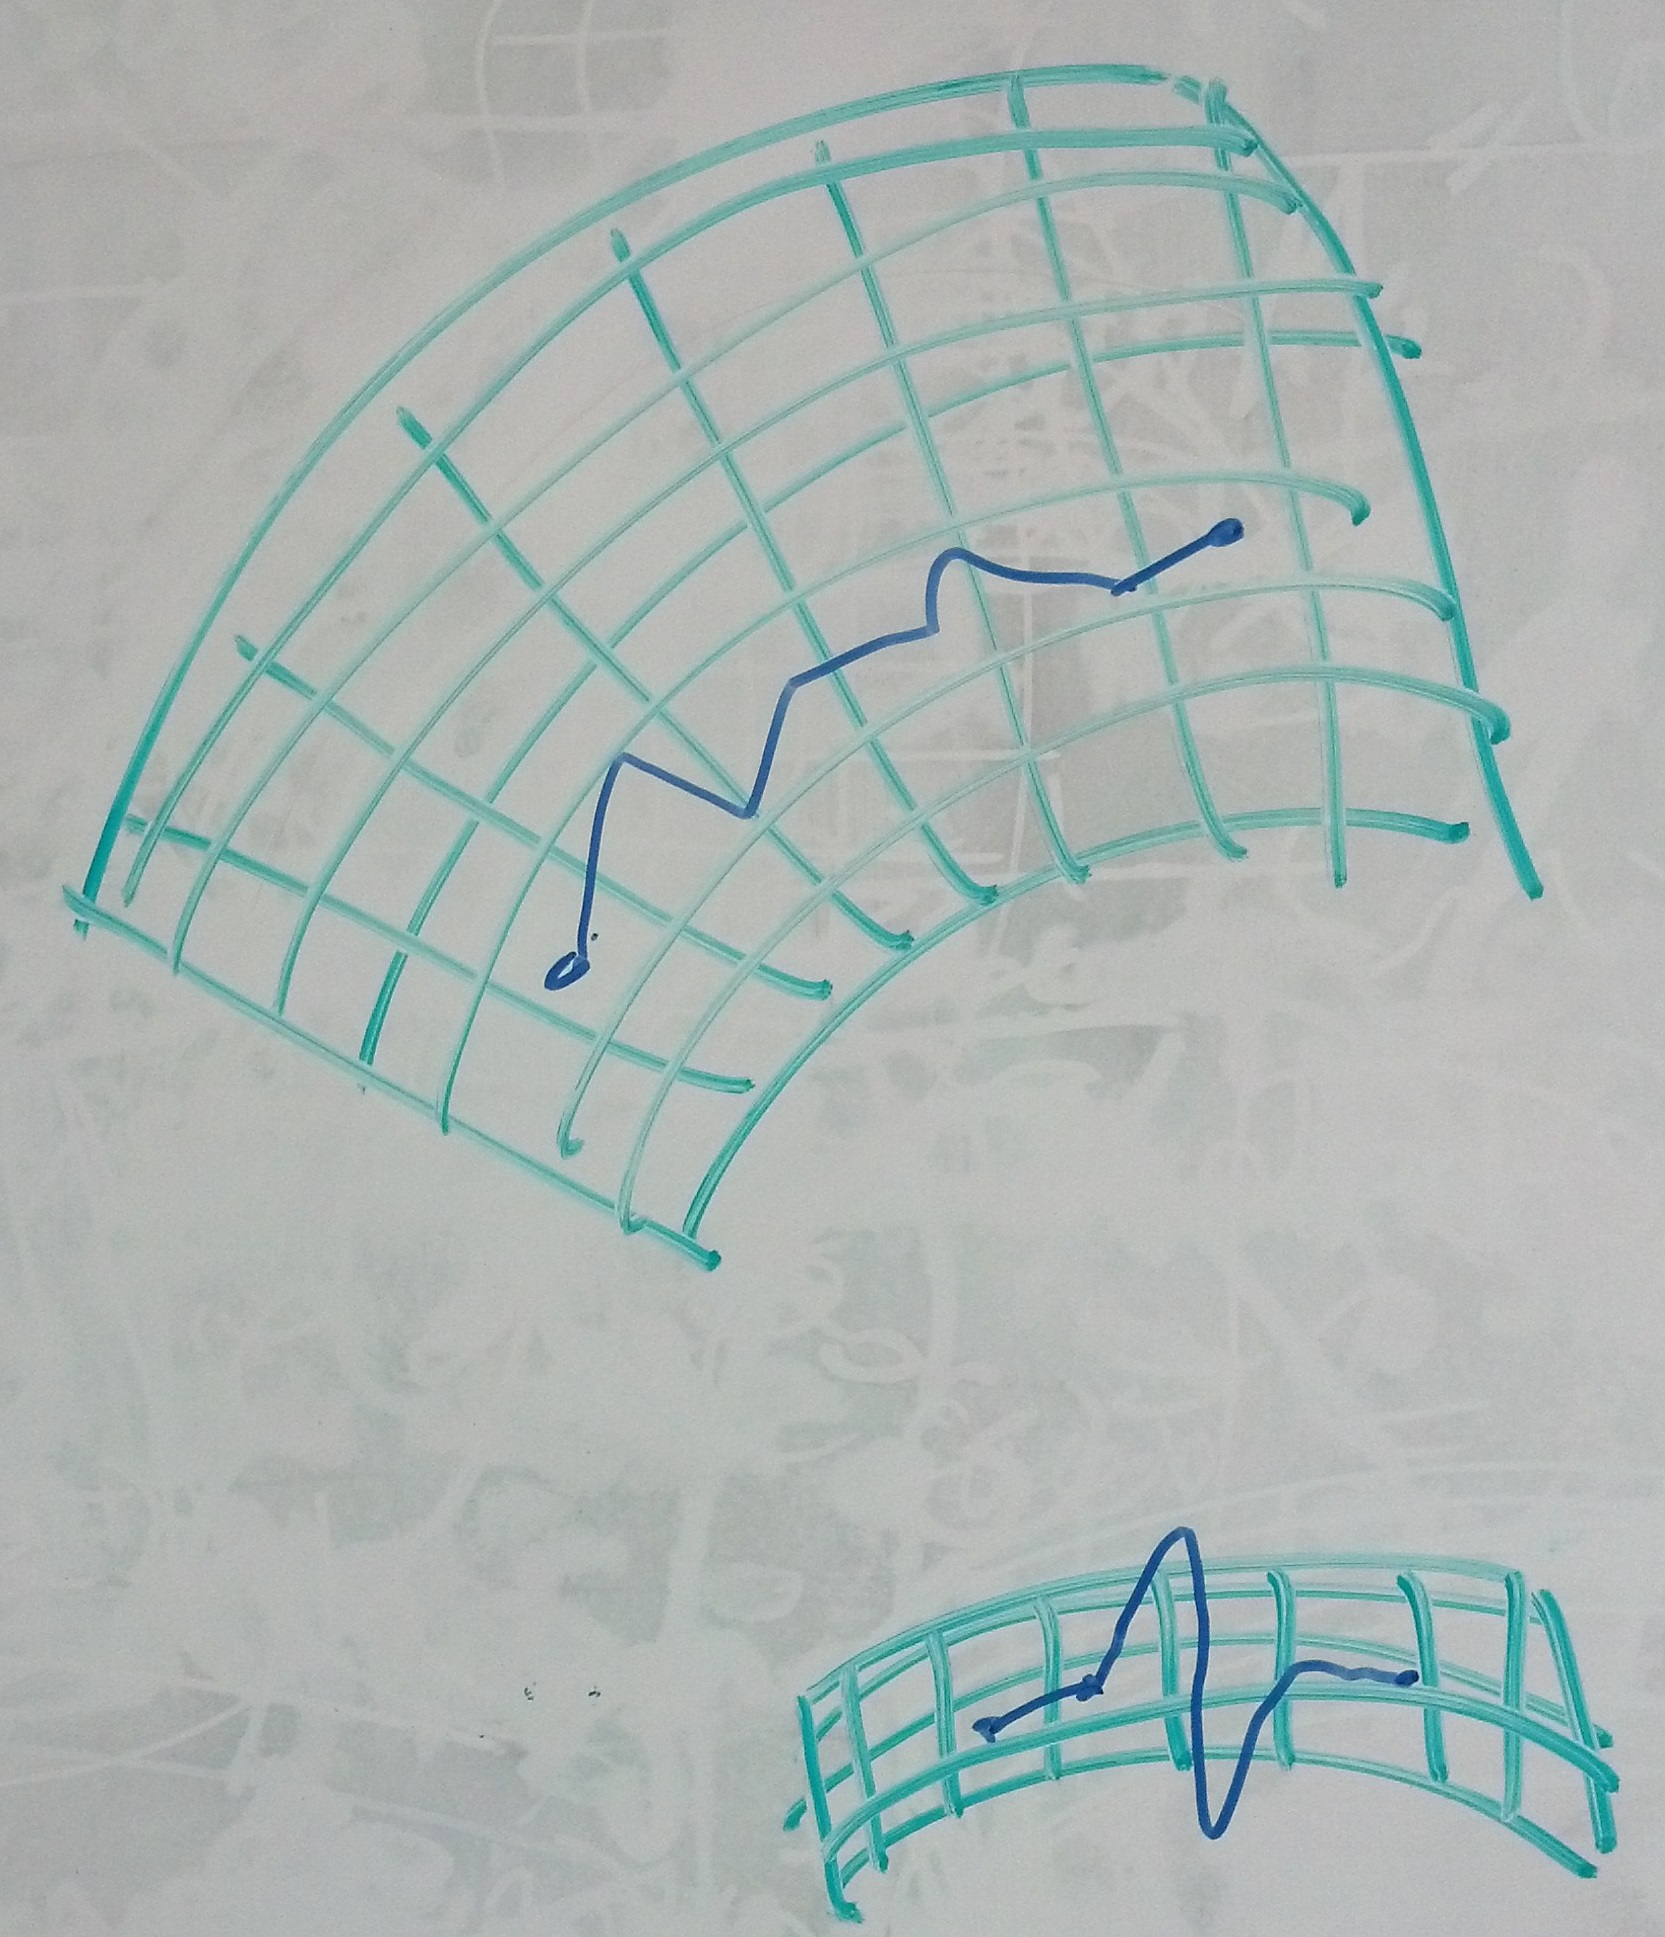
\includegraphics[width=\columnwidth]{pathaboveandbelow.jpg}
\caption{Path above and below surface}
\label{pathsAboveAndBelow}
\end{figure}

We have a known and rigid starting point $p_0$ on the triangular manifold mesh $M$ for our path (TODO: The fact that it is a triangular manifold mesh will be established in previous sections). The rest of the path is a set of $n$ segments $s_0,...,s_{n-1}$ where the starting point of $s_0$ is $p_0$ and the rest of the segments start at the point where the previous segment ended. We need a new set of segments that all lie on triangles of the mesh. Our goal is thus a new path consisting of $m$ points, $p_0, p_1,...,p_{m-1}$, such that each $p_i$ is on $M$ and for each $i>0$, $p_{i}$ and $p_{i-1}$ lie on the same triangle. \\
\\
Once the first segment is transformed to follow the mesh, we will have a new point $p_j$ on the mesh where the first segment ends and the second segment begins. Because each segment starts where the previous one ended, we will transform the second segment using $p_j$ as its starting point. By this same logic, we can repeat this procedure for the rest of the segments. We thus need to focus now on how to transform a single segment with a starting point to points on the mesh making sure to preserve length and orientation along the surface. \\
\\
When we transform a segment, it needs to follow a straight-line path in its direction for its length, thus it should follow the geodesic path along the surface. We will therefore flatten the mesh around the local area that the segment traverses. Let $\epsilon$ be the length of our segment and $p$ be its starting point. The $\epsilon$-neighborhood around $p$ will be homeomorphic to $R^2$, as illustrated in Figure \ref{manifolddiagram}, thus when we flatten the neighborhood, there will be no gaps or overlaps. We will denote $T$ as the triangle where the starting point lies. We will develop a secondary mesh $M_0$ that consists of $T$ and the triangles that intersect the $\epsilon$-neighborhood of $T$. The triangles in $M_0$ will be rotated so that they lie on the same plane as $T$. \\
\\
We now have a vector and a flat plane it needs to follow. We will let $v$ be the vector for our input segment, $N$ be the normal of that plane. In order to preserve orientation along the plane, we need to find a vector $E$ that is both on the plane formed by $N$ and $v$ and has an acute angle with $v$. As can be observed in figure \ref{vectordiagram}, the following equation will then hold
\[
E + proj_N(v) = v
\]

\begin{figure}[ht]
\centering
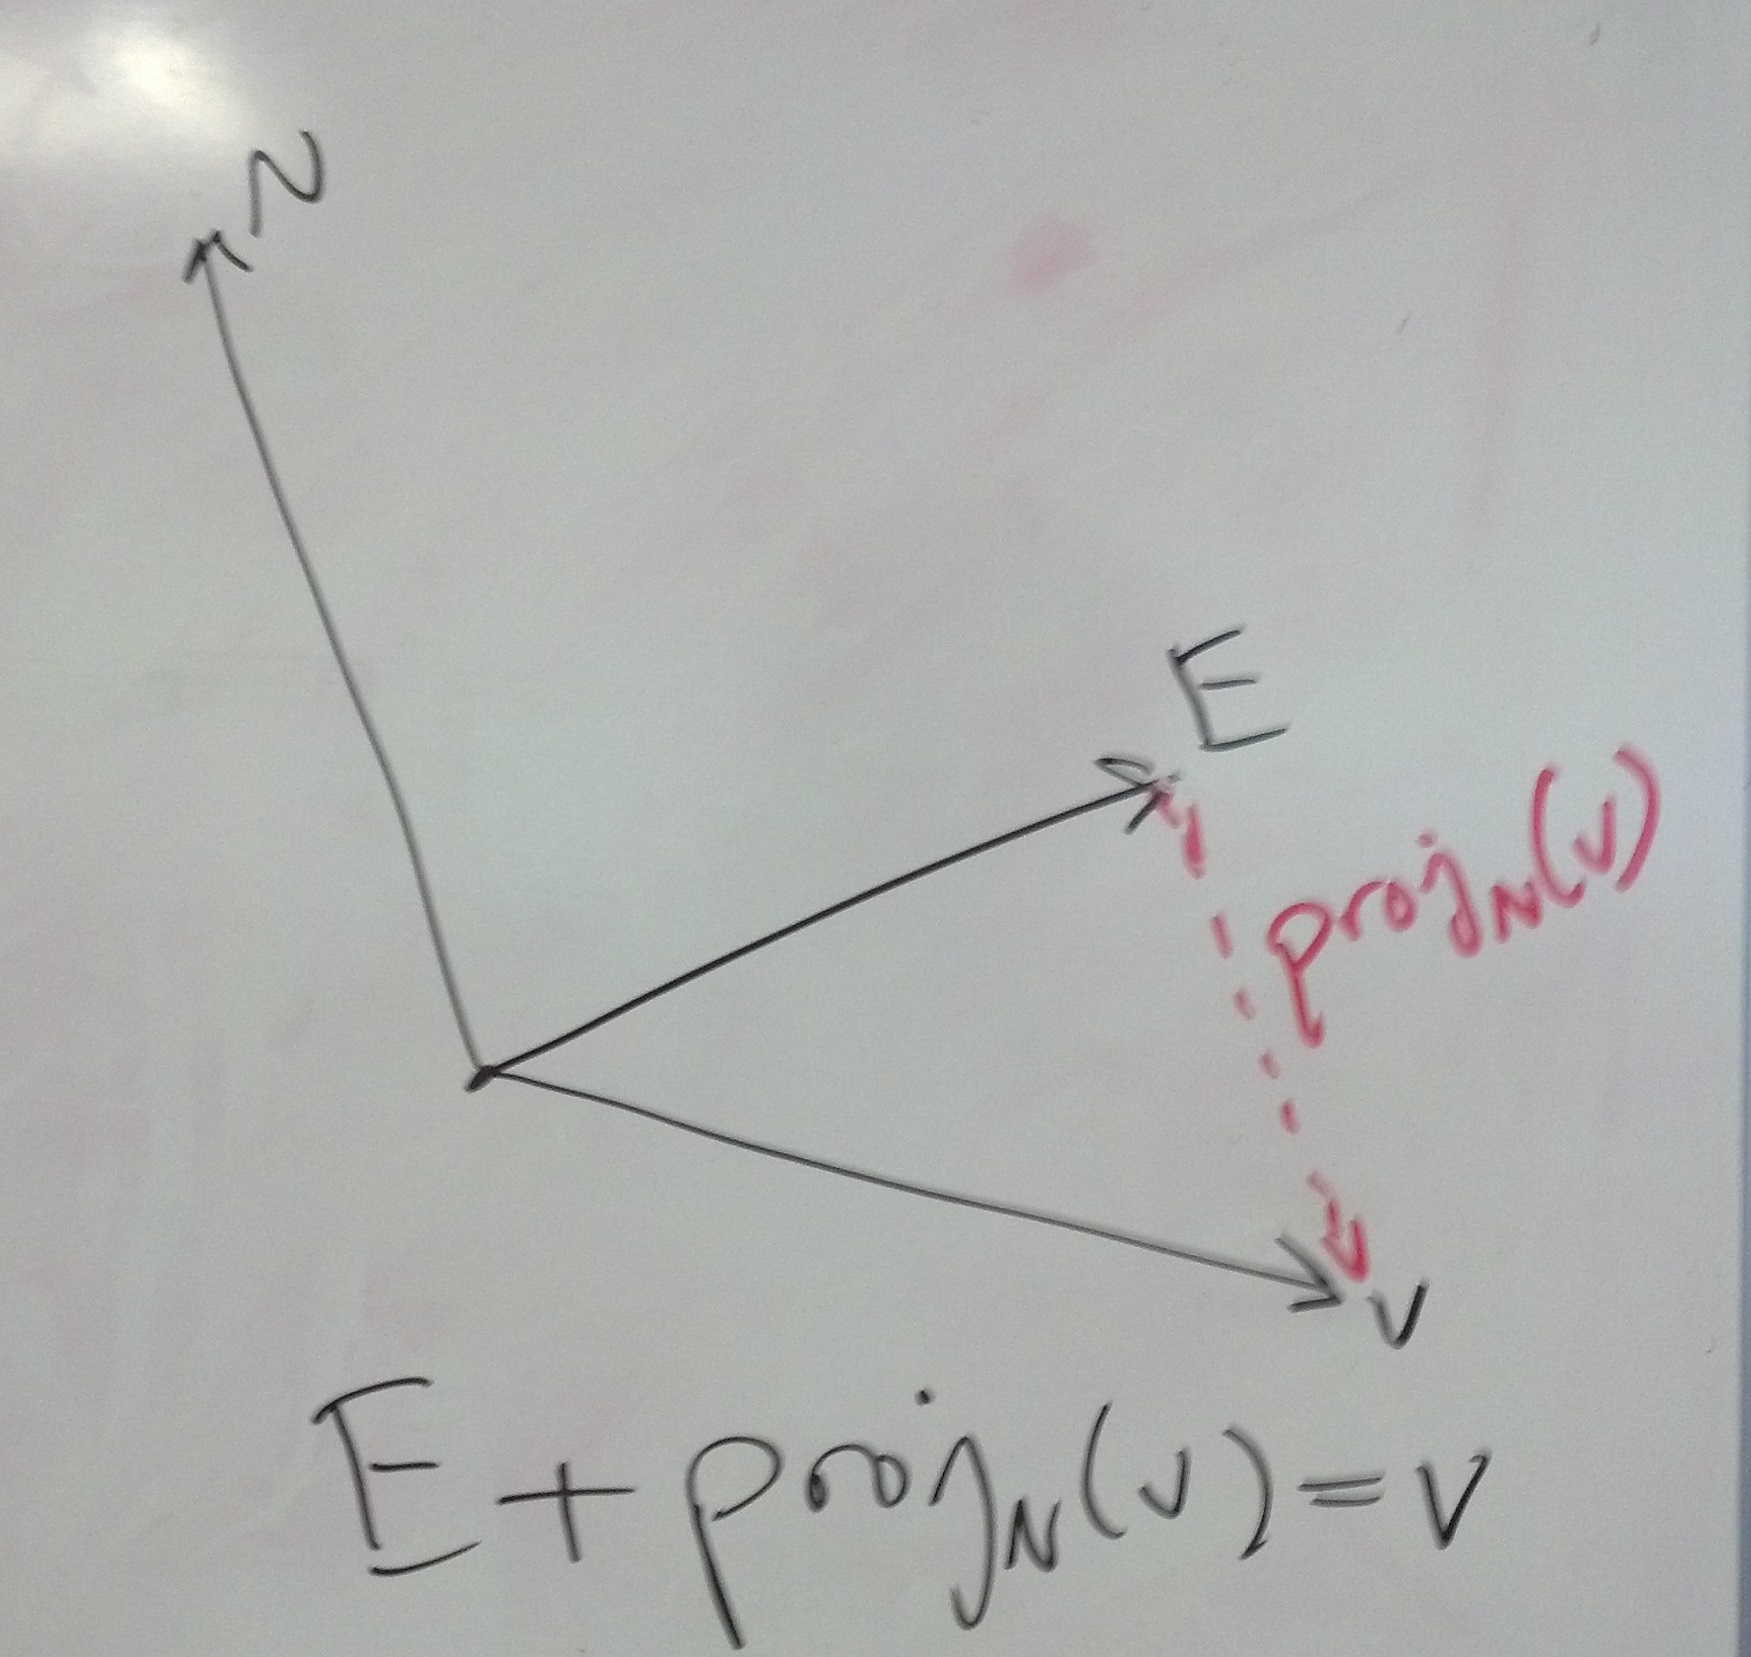
\includegraphics[width=\columnwidth]{vectordiagram.jpg}
\caption{The segment vector, normal, and projected vector}
\label{vectordiagram}
\end{figure}

Thus we can easily calculate $E$ using the formula
\[
E = v - N(v.N)
\]
We will now let $p' = p+E$ which will be the ending point on $M_0$ of our segment. We then take the $p-p'$ line segment and calculate its intersections with edges of the triangles in $M_0$, denoting that set as $Q'$. The points $p$ and $p'$ will also be calculated in their own triangle's coordinate system. The points in $Q'$ that lie on edges between triangles will be calculated in the coordinate systems of both triangles. By finding the point coordinates in the triangle's coordinate system, we can easily transform the $p-Q'-p'$ set of points into the set $\{p_0,...,p_j\}$ where each of those points lie on the mesh $M$. As a summary, the pseudo-code of the algorithm is presented in algorithm \ref{pseudocode}. \\
\\
\begin{algorithm}[t]
Input: Starting point $p_0$, Segments $s_0,...,s_m$, Mesh $M$\;
Set $p \leftarrow p_0$ \;
Initialize list $P$ of points and add $p_0$ to it \;
Set $T$ to be the triangle of $p_0$ \;
\For{each segment $s_i$ in order}{
	Set $N$ to be normal for $T$\;
	Set $\epsilon \leftarrow length(s_i)$ \;
	Set $M_0$ equal to triangles which intersect the $\epsilon$-neighborhood around $p$ \;
	Flatten $M_0$ so its global normal is $N$ \;
	Set $v$ to be the vector for $s_i$ \;
	Set $E \leftarrow v - N(v.N)$ \;
	Set $p' \leftarrow p+E$ \;
	Set $Q'$ to be intersections of $p-p'$ segment with triangle edges in $M_0$ \;
	Transform $p$,$Q'$,$p'$ back to points on M and add them to $P$ \;
	Set $p$ to transformed $p'$. \;
	Set $T$ to triangle at $p'$ \;
}
\caption{Pseudo-code for our algorithm}
\label{pseudocode}
\end{algorithm}

\begin{figure}[ht]
\centering
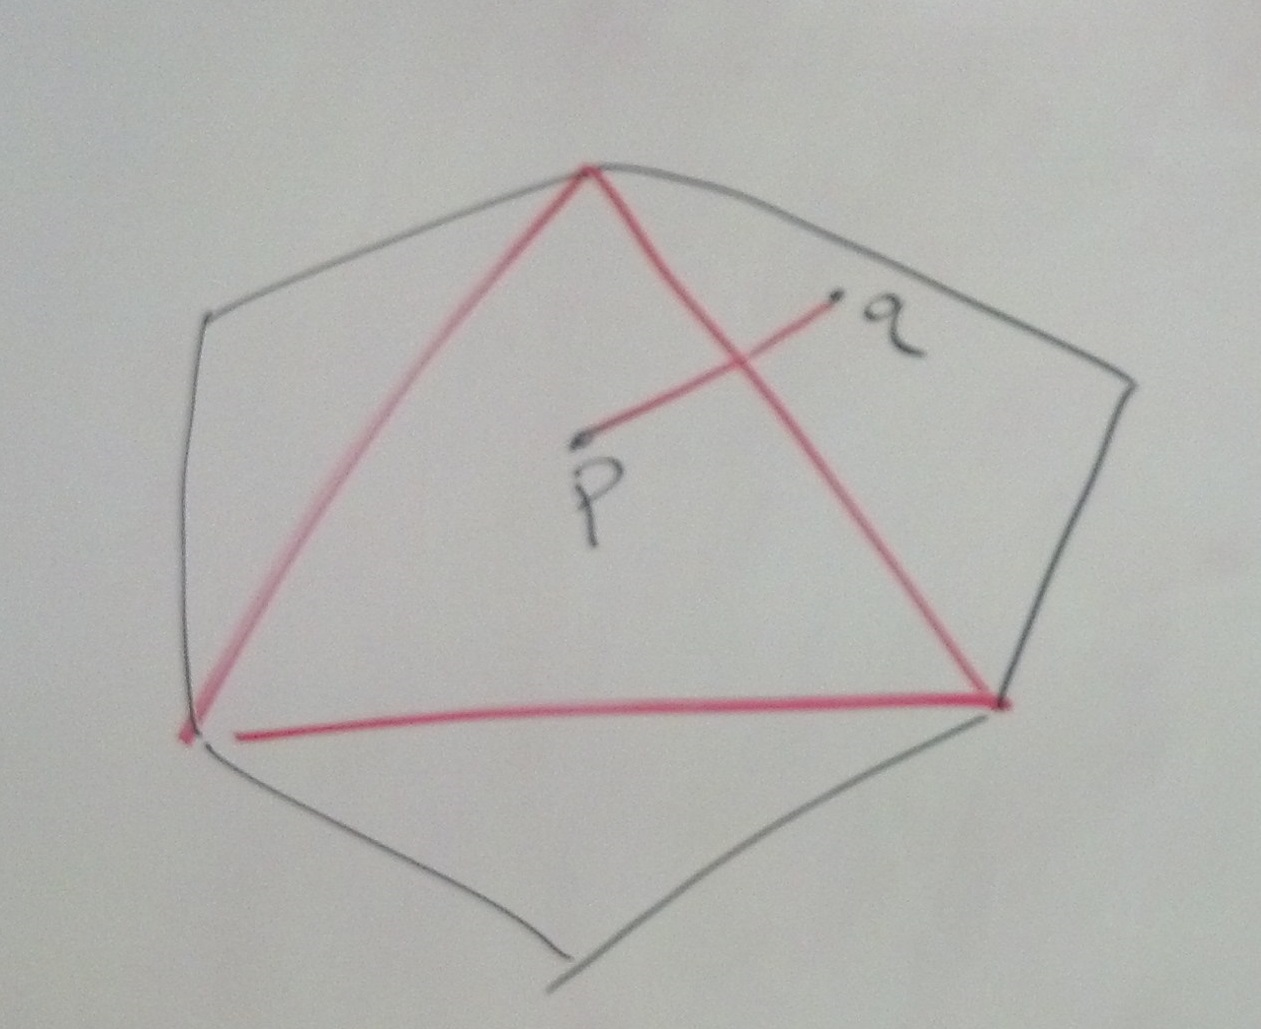
\includegraphics[width=\columnwidth]{flatteningdiagram_oneTriangleAndNeighbors.jpg}
\caption{The triangle at $p$ and its neighbors}
\label{flatteningDiagram_oneTriangle}
\end{figure}
\begin{figure}[ht]
\centering
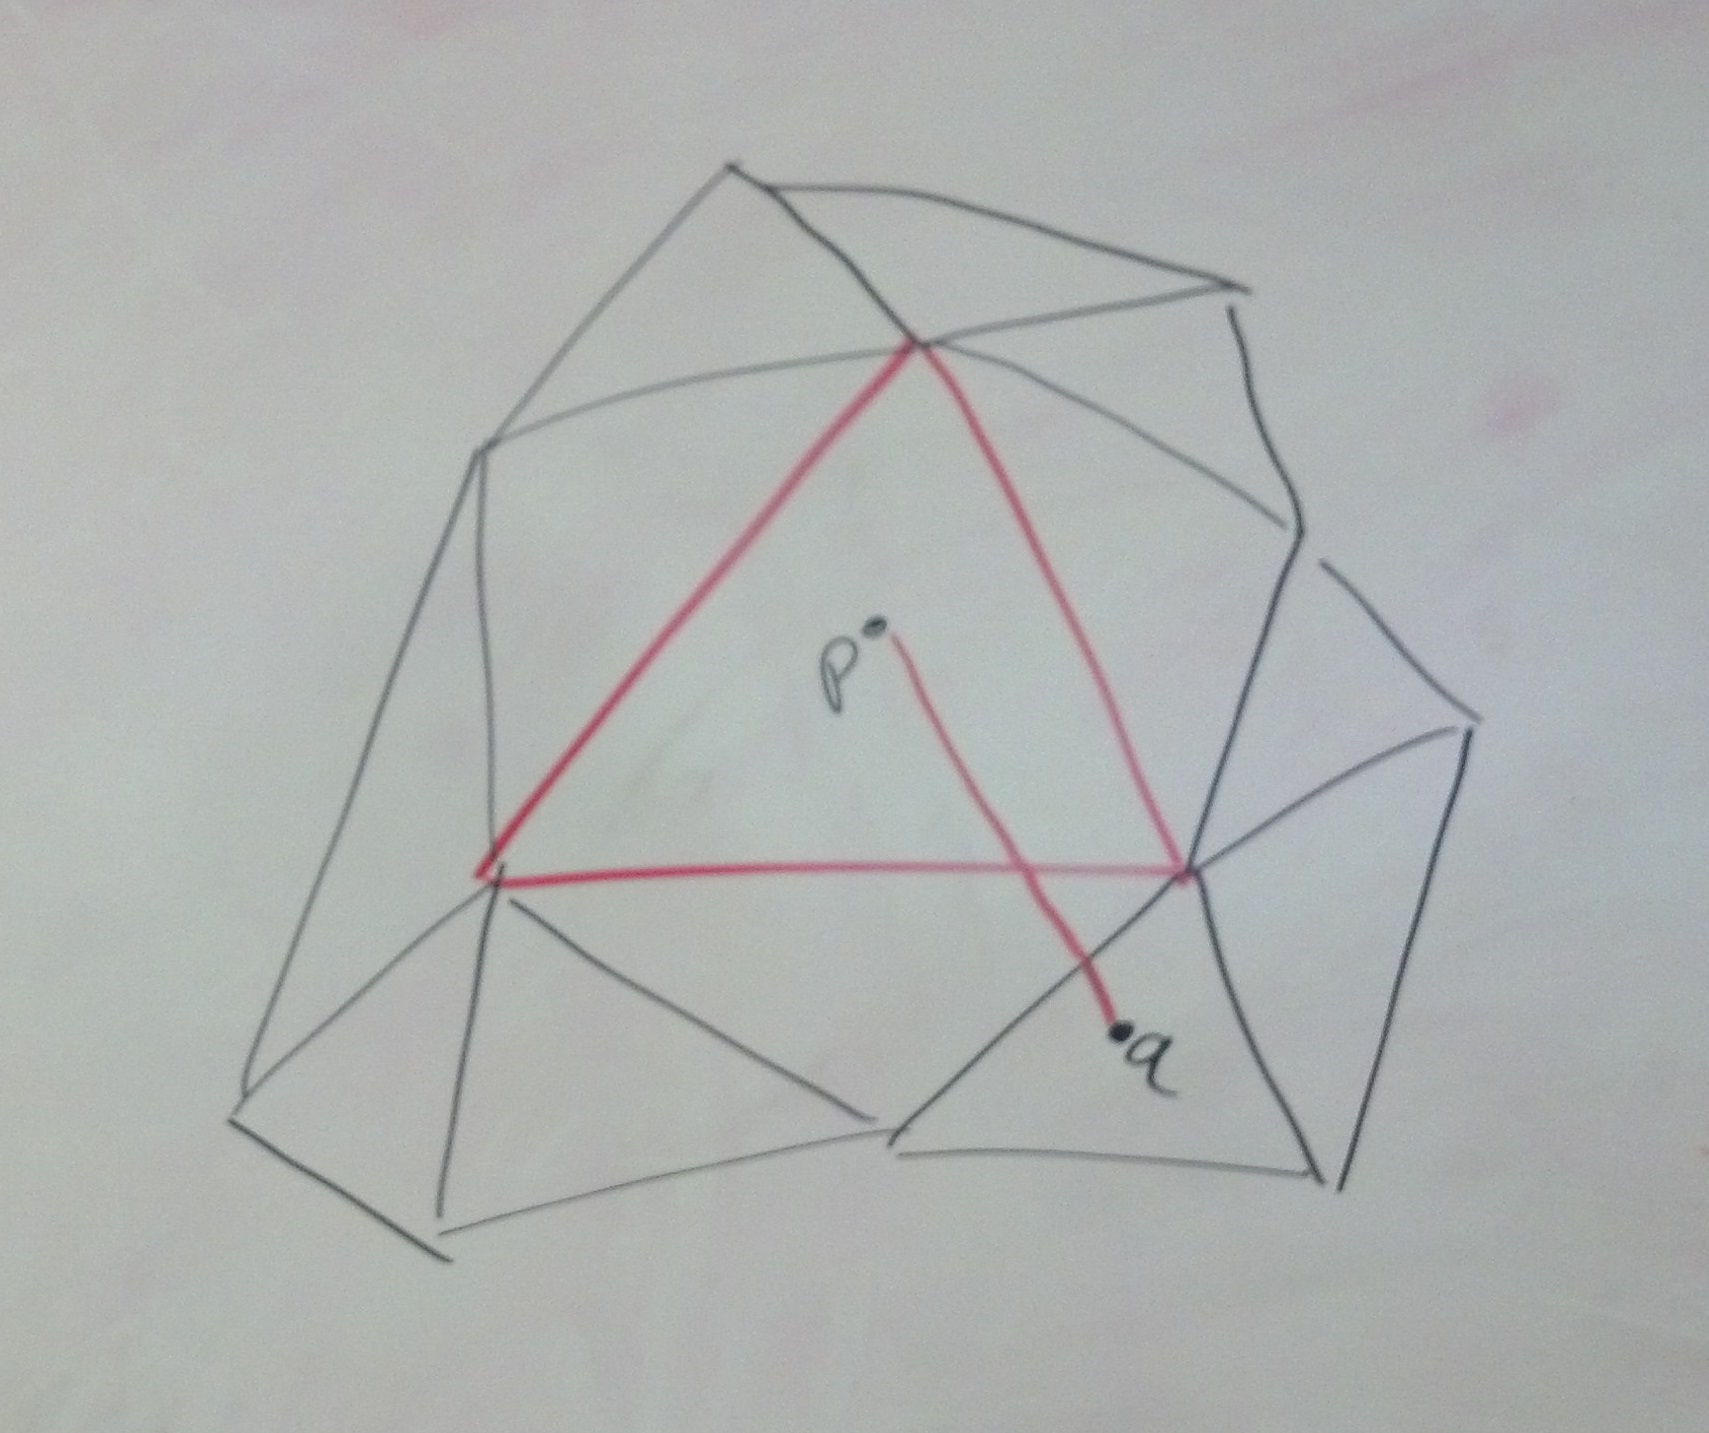
\includegraphics[width=\columnwidth]{flatteningdiagram_neighborhood.jpg}
\caption{The triangles in the neighborhood around $p$}
\label{flatteningDiagram_neighborhood}
\end{figure}

\begin{figure}[ht]
\centering
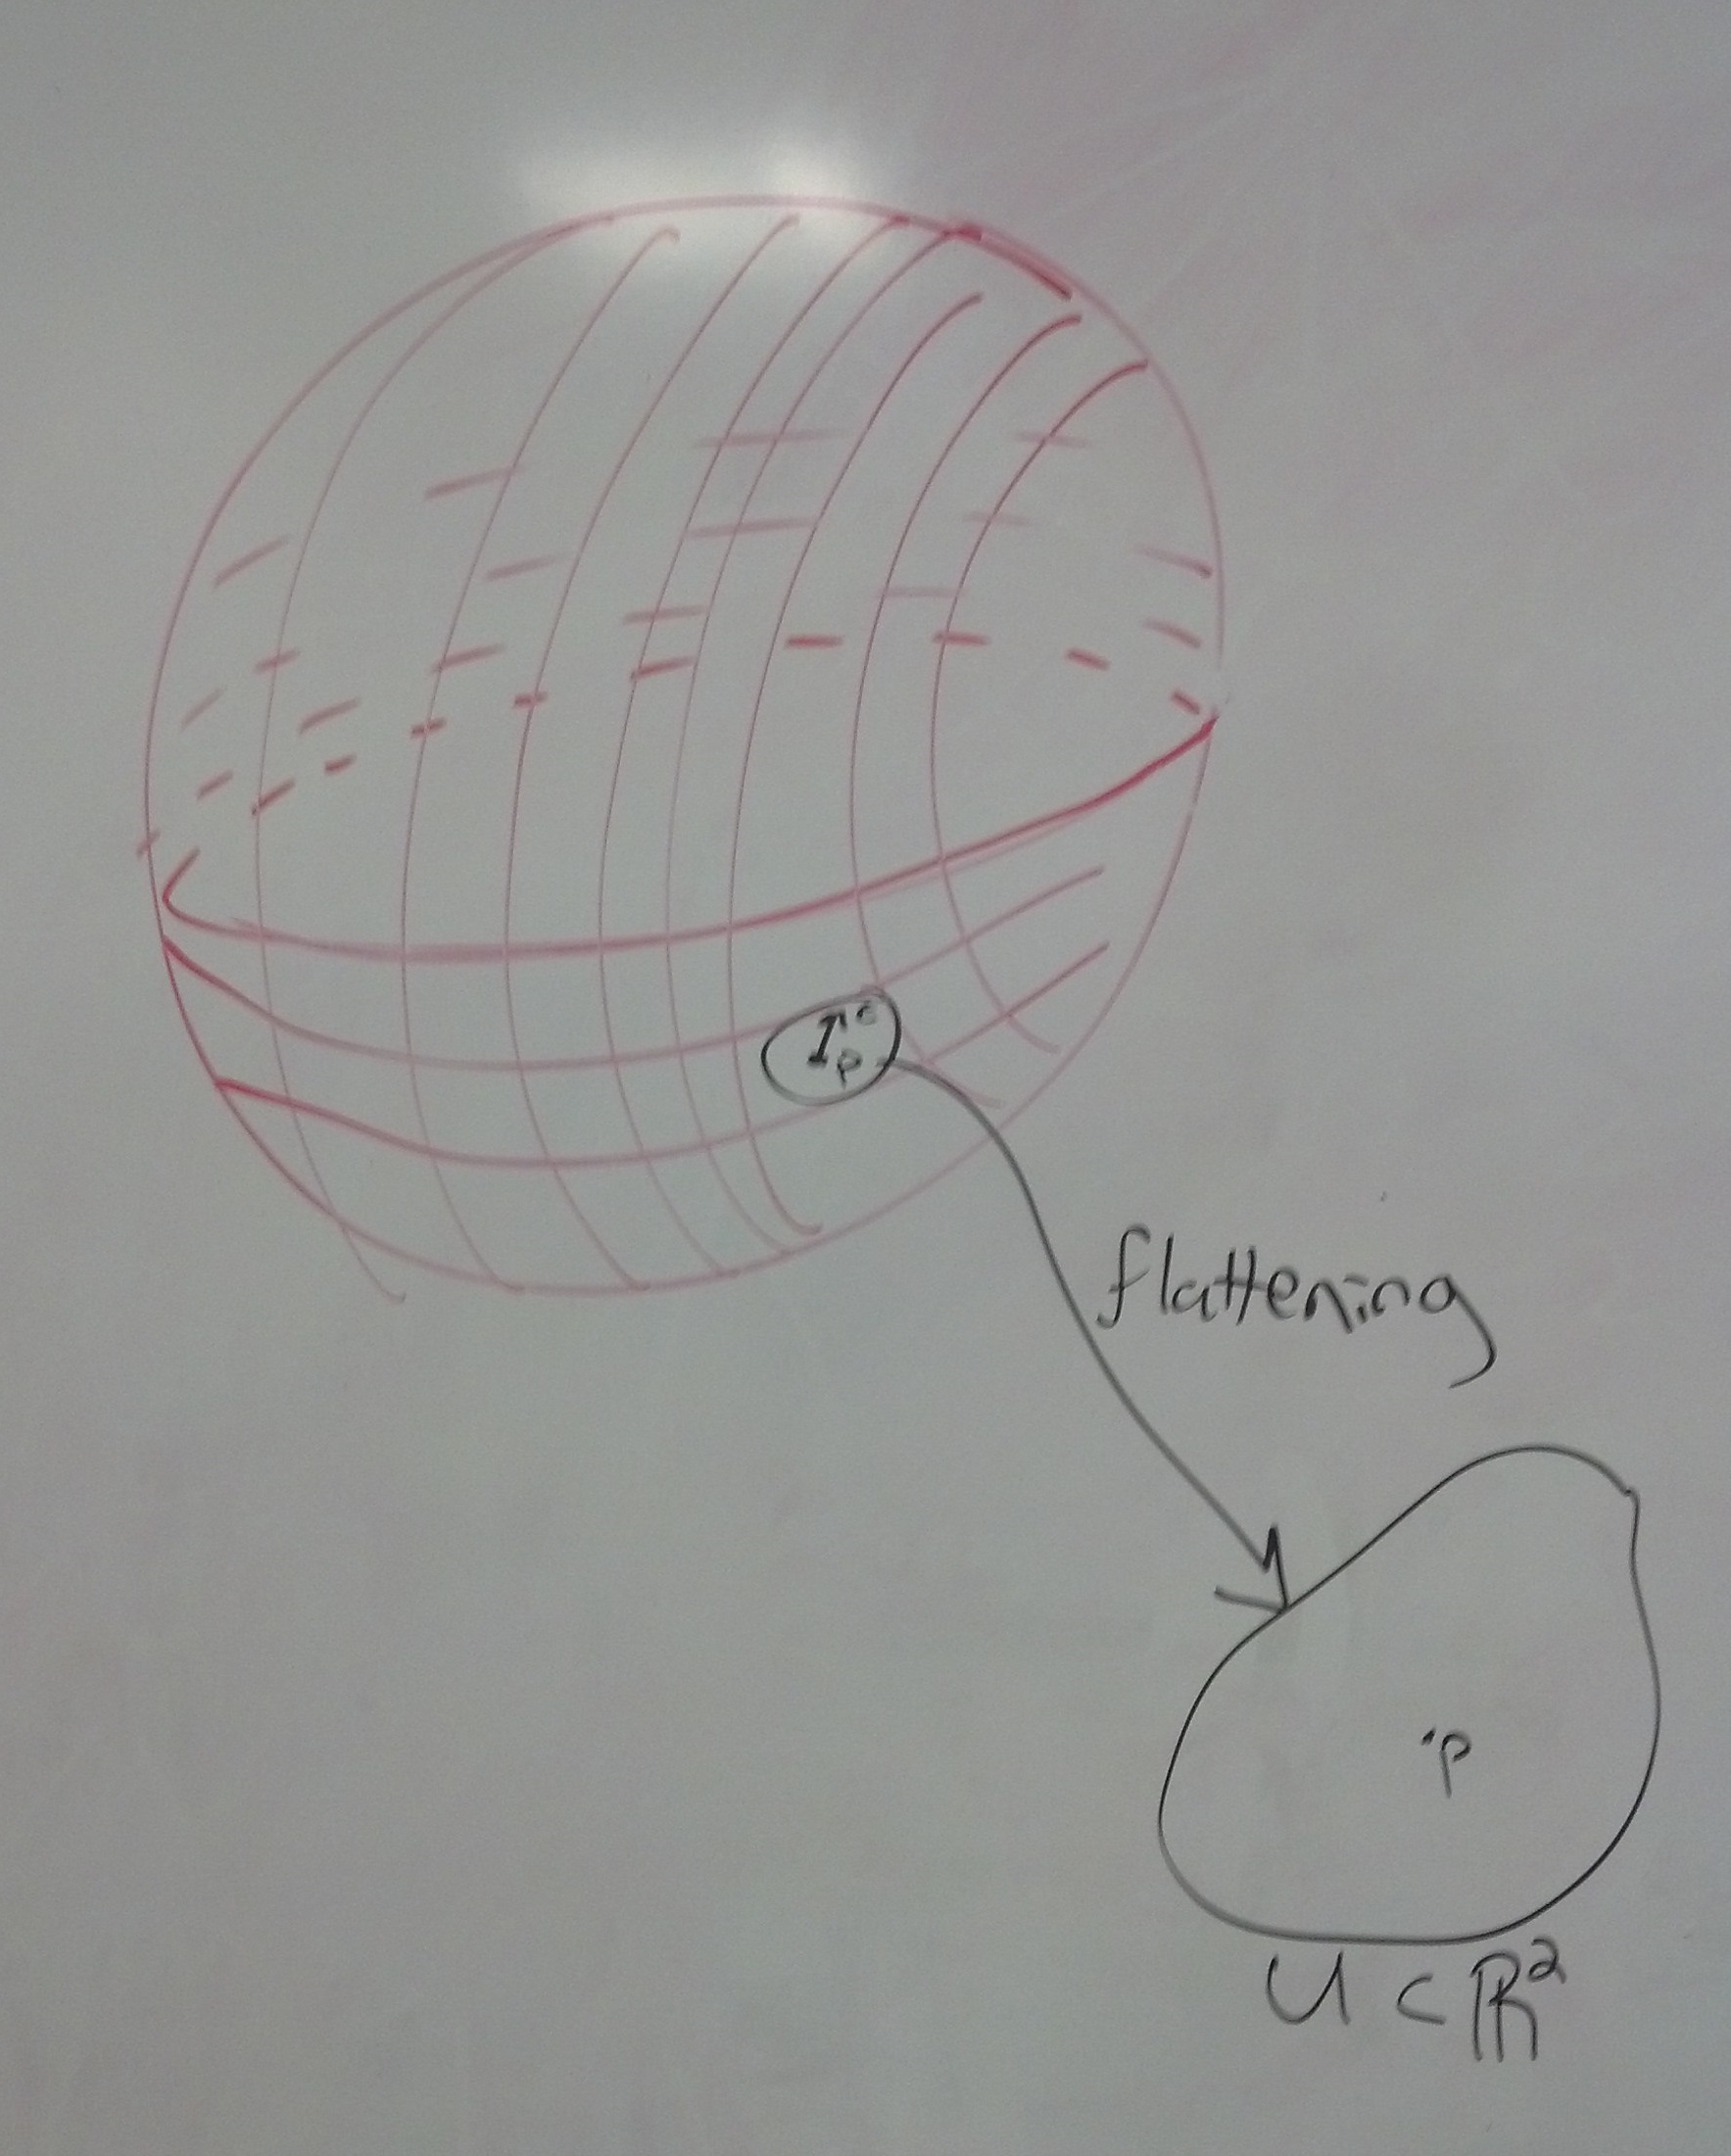
\includegraphics[width=\columnwidth]{manifolddiagram.jpg}
\caption{The manifold with its $\epsilon$ neighborhood at a point $p$}
\label{manifolddiagram}
\end{figure}
